\section{Docker's Swarm:}
\label{sec:swarm}
Docker Swarm is Docker’s native clustering tool that allows to make a group of Docker engines into a single, virtual Docker Engine. This allows the services to scale out as if they are running on a single machine with large resources. Swarm allows to get rid of the trouble of deciding the nodes where to start the docker containers. Although docker swarm is a clustering tool, but the definition of cluster is limited to the pool of Docker engines. 

\begin{figure*}
\centering
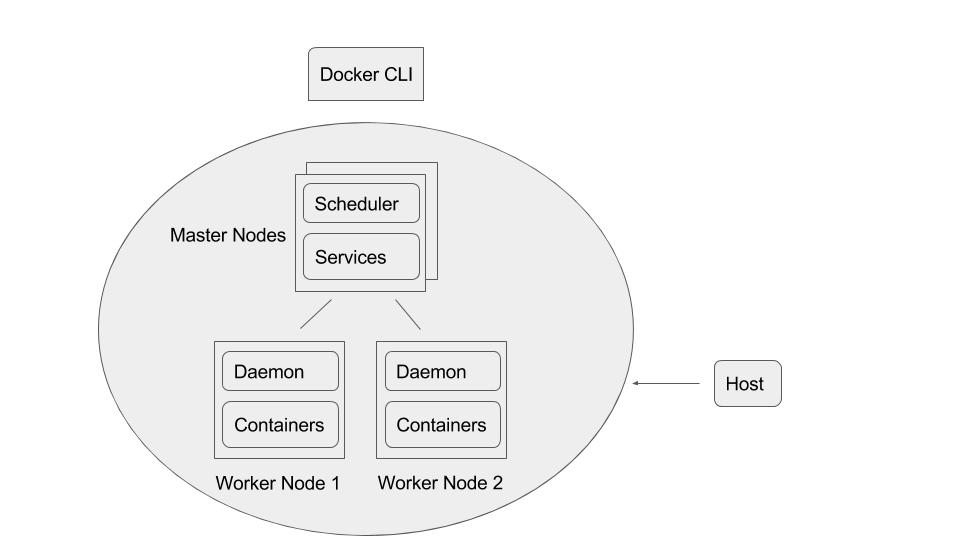
\includegraphics[scale=0.5]{./fig/swarm}
\caption{Docker Swarm Architecture}
\label{fig:swarmArch}
\end{figure*}

To create a swarm of Docker’s engine, it first requires steps of
\begin{itemize}
\item defining the cluster,
\item joining of hosts to the cluster and,
\item creating the cluster manager. 
\end{itemize}
Hosts become nodes after they join the swarm. These nodes are classified as manager nodes and worker nodes in Swarm. Manager nodes are responsible for the scheduling, coordination and managing the resources of swarm nodes.

Worker node’s job is to run the tasks which are forwarded by the manager node to them. By default, all manager nodes are worker nodes. Docker Swarm selects one of these  manager nodes as primary that manages the swarm, does scheduling and launches the tasks to a worker node in container. 

Following are the features of Swarm:
\begin{enumerate}
\item Compatibility with Docker APIs:
Swarm uses the standard Docker APIs. This allows any services or applications, which were using Dockers, to scale out to multiple nodes. Swarm’s use of Docker’s API make it easy to use. However, this makes Swarm to inherit the constraint of Docker’s APIs. 

\item High availability:
High availability in swarm is achieved by having multiple instances of the manager node. The primary manager talks to the nodes of the cluster. If the primary manager fails, one of the other instance of the manager node will replace it and will become the primary manager node.

\item Pluggable schedulers:
Although swarm has its own scheduler, but it is optional. Swarm allows to use third party schedulers like Mesos by using the plugin while running the tasks using Docker clients.  This follows the Docker philosophy of “batteries included but removable.”

\item Node Labeling:
One of the most powerful features of swarm is labeling of the nodes. Like Kubernetes, Swarm allows the users to put custom label in the nodes. The labeling of nodes allows the users to constrain which nodes a container can start on. Swarm also allows to tag a node with multiple labels. This allows the user to put more broad constraints on a container.

\item Container Affinity:
In some cases, the placement of a container must be relative to other containers. Swarm lets you define those relationships through affinities. Affinities are automatically generated when the relationship between containers is implied.

\item Swarm Discovery:
Swarm can use hosted discovery service, static file, etcd, consul or zookeeper for the service discovery.

\item TLS:
TLS authentication can be enabled to secure the communication to and from Swarm.

\item Integrated networking and Volumes:
Since Swarm is a Docker’s native tool, it can use Docker Networking, Volumes and plugins through their respective Docker commands.


\item Flexible Scheduling:
In addition to labeling and affinity features, multiple scheduling strategies like spread and binpack gives the flexibility to assign the container to a specific node maximizing the resource utilization.


\item High Scalability:
In production environment, Swarm’s performance has been tested up to 50000 containers without any performance drop. 

\end{enumerate}